%% ======================================================================
%% APPENDIX — Sun-Synchronous Orbit Analysis and RGTO Comparison
%% ======================================================================
\chapter{Comparison between Sun-Synchronous Orbit and Repeating Ground Track Orbit}
\label{app:sso_orbit}

This appendix develops the astrodynamic theory of the Sun-Synchronous Orbit (SSO) and presents a quantitative comparison between the SSO and the Repeating Ground Track Orbit (RGTO) seed adopted in the main text.  The SSO is included as a commercially motivated comparison baseline: it is the predominant LEO orbit class for Earth observation, and its widespread availability via rideshare launches makes it the natural benchmark against which the mission-specific RGTO design is evaluated.

%% ------------------------------------------------------------------
\section{Sun-Synchronous Orbit (SSO)}
\label{72-SSO_intro}
%% ------------------------------------------------------------------

A \textbf{Sun-Synchronous Orbit} (SSO) is a near-polar, retrograde orbit ($i > 90^{\circ}$) whose orbital plane precesses eastward at exactly the rate at which the Earth revolves around the Sun, therefore maintaining a constant angle between the orbital plane and the Earth--Sun direction throughout the year.  This property guarantees repeatable solar illumination conditions at each latitude crossing, making SSOs the predominant choice for optical and multispectral Earth-observation missions. This section defines the equations used to model SSO to create a comparison with the RGTO case. The equations are based on Vallado's book \cite{valladoFundamentalsAstrodynamicsApplications2001}.

\subsection{Sun-Synchronous Condition}
\label{sec:sso_condition}

The SSO condition requires that the secular nodal regression rate $\dot{\Omega}$ (Eq.~\eqref{eq:dot_Omega}) matches the mean angular velocity of the Earth's orbital motion around the Sun:
\begin{equation}
    \dot{\Omega}_{\mathrm{SSO}} = \frac{2\pi}{T_{\odot}} \approx 1.991 \times 10^{-7}\;\mathrm{rad\,s^{-1}},
    \label{eq:sso_omega_dot}
\end{equation}
where $T_{\odot} = 365.2421897\;\mathrm{d}$ is the mean tropical year.  Substituting Eq.~\eqref{eq:dot_Omega} into this condition yields the fundamental SSO design equation relating $a$, $e$, and $i$:
\begin{equation}
    -\frac{3}{2}\,J_2 \left(\frac{R_{\oplus}}{p}\right)^{\!2} \sqrt{\frac{\mu_{\oplus}}{a^3}}\,\cos i \;=\; \dot{\Omega}_{\mathrm{SSO}},
    \label{eq:sso_fundamental}
\end{equation}
where $p = a(1 - e^2)$ is the semi-latus rectum.  Because the required nodal precession is eastward ($\dot{\Omega} > 0$) and $\dot{\Omega} \propto -\cos i$, the cosine of the inclination must be negative, constraining $i > 90^{\circ}$ (retrograde orbit).

\subsection{Inclination from Semi-Major Axis}
\label{sec:sso_inc_from_a}

For a given semi-major axis $a$ and eccentricity $e$, solving Eq.~\eqref{eq:sso_fundamental} for inclination yields~\cite[Eq.~11-15]{valladoFundamentalsAstrodynamicsApplications2001}:
\begin{equation}
    i_{\mathrm{SSO}} = \arccos\!\left(-\frac{2\,\dot{\Omega}_{\mathrm{SSO}}\,a^{7/2}\,(1 - e^2)^2}{3\,J_2\,R_{\oplus}^2\,\sqrt{\mu_{\oplus}}}\right).
    \label{eq:sso_inclination}
\end{equation}
This expression is the primary design equation used to define a SSO: given $a$ and $e$, the sun-synchronous inclination is uniquely determined.

\subsection{Semi-Major Axis from Inclination}
\label{sec:sso_a_from_inc}

Conversely, if the inclination is prescribed, the required semi-major axis is obtained by rearranging Eq.~\eqref{eq:sso_fundamental}~\cite[Eq.~11-14]{valladoFundamentalsAstrodynamicsApplications2001}:
\begin{equation}
    a_{\mathrm{SSO}} = \left(\frac{-3\,J_2\,R_{\oplus}^2\,\sqrt{\mu_{\oplus}}\,\cos i}{2\,\dot{\Omega}_{\mathrm{SSO}}\,(1 - e^2)^2}\right)^{\!2/7}.
    \label{eq:sso_sma}
\end{equation}

\subsection{Eccentricity from Semi-Major Axis and Inclination}
\label{sec:sso_ecc}

When both $a$ and $i$ are fixed, the eccentricity compatible with the sun-synchronous condition follows from~\cite[Eq.~11-16]{valladoFundamentalsAstrodynamicsApplications2001}:
\begin{equation}
    e_{\mathrm{SSO}} = \sqrt{1 - \sqrt{\frac{-3\,J_2\,R_{\oplus}^2\,\sqrt{\mu_{\oplus}}\,\cos i}{2\,a^{7/2}\,\dot{\Omega}_{\mathrm{SSO}}}}}\,.
    \label{eq:sso_ecc}
\end{equation}
Equations~\eqref{eq:sso_inclination}--\eqref{eq:sso_ecc} form a closed system: specifying any two of $(a,\,e,\,i)$ uniquely determines the third under the SSO constraint.

\subsection{RAAN and Local Time of the Ascending Node (LTAN)}
\label{sec:sso_ltan}

A defining operational parameter of any SSO is the \textbf{Local Time of the Ascending Node} (LTAN), which specifies the local solar time at which the satellite crosses the equator northbound.  Given a reference epoch $t_0$ and the Sun's apparent right ascension $\alpha_{\odot}(t_0)$ at that epoch, the RAAN required to achieve a desired LTAN is:
\begin{equation}
    \Omega_{\mathrm{SSO}} = \alpha_{\odot}(t_0) + \bigl(\mathrm{LTAN}_{\mathrm{h}} - 12\bigr) \times 15^{\circ},
    \label{eq:sso_raan_ltan}
\end{equation}
where $\mathrm{LTAN}_{\mathrm{h}}$ is the LTAN expressed in hours.  Common choices include $\mathrm{LTAN} = 06\!:\!00$ (dawn--dusk, minimal shadow) and $\mathrm{LTAN} = 10\!:\!30$ (morning descending node with favourable illumination for optical imaging).

\subsection{SSO Orbital Element Vector}
\label{sec:sso_element_vector}

Analogously to the RGTO element vector (Eq.~\eqref{eq:rgto_element_vector}), the SSO orbit of satellite $S_k$ is fully specified by:
\begin{equation}
    \vec{\mathbf{A}}^{\,\mathrm{SSO}}{}_{k} = \bigl[a,\; e,\; i_{\mathrm{SSO}},\; \omega,\; \Omega,\; \nu,\; t_0\bigr]^{T},
    \label{eq:sso_element_vector}
\end{equation}
where $i_{\mathrm{SSO}}$ is obtained from Eq.~\eqref{eq:sso_inclination}.  Unlike the RGTO, where the period ratio $\tau$ replaces $a$ as the independent design parameter, in the SSO the semi-major axis $a$ remains the primary free parameter because the inclination is uniquely determined by the sun-synchronous condition for a given $(a, e)$ pair.

%% ------------------------------------------------------------------
\section{SSO Seed Orbit Parameters}
\label{sct-SSO_seed}
%% ------------------------------------------------------------------

The SSO seed orbit is selected to represent the most operationally accessible orbit class for LEO Earth observation.  The majority of small-satellite launches to LEO utilise rideshare services on reusable launch vehicles, such as SpaceX Falcon~9 Transporter mission, which inject payloads into a common SSO defined by the launch provider's target semi-major axis and epoch.  This shared-ride operation makes the SpaceX rideshare SSO the reference orbit for cost-constrained LEO missions. Therefore, we adopt this orbit as the SSO baseline, ensuring a comparison with the RGTO seed and reflecting a realistic, commercially available alternative.

As explained in Section~\ref{72-SSO_intro}, the SSO seed is completely determined by two independent parameters: the semi-major axis $a$ and the insertion epoch~$t_0$.  Given these, the $J_2$-driven sun-synchronous condition (Eq.~\eqref{eq:sso_inclination}) defines the inclination $i_{\mathrm{SSO}}$ such that the secular nodal regression rate $\dot{\Omega}$ (Eq.~\eqref{eq:dot_Omega}) exactly compensates the apparent motion of the Sun, maintaining a constant orbital-plane orientation with respect to the Earth--Sun line throughout the year.

Using as example the SpaceX Transporter injection parameters ($a = 6904$\,km, $e = 0.0$, epoch 2021-01-24T15:00\,UTC), the SSO conditions  (Sec.~\ref{sec:sso_condition}) yields the SSO seed orbital element vector:
\begin{equation}
    \vec{\mathbf{A}}^{\,\mathrm{SSO}}{}_{0} = \bigl[6904\;\mathrm{km},\; 0.0,\; 97.50^{\circ},\; 0^{\circ},\; 0^{\circ},\; 0^{\circ},\; t_0\bigr]^{T},
    \label{eq:sso_seed_vector}
\end{equation}
where $t_0 = \text{2021-01-24T15:00 UTC}$.  Table~\ref{tab:sso_seed_parameters} summarises the complete set of derived parameters for this seed orbit.

\begin{table}[H]
\centering
\caption{\footnotesize{SSO seed orbit parameters derived from the SpaceX Transporter rideshare injection conditions ($^{\ddagger}$).  The inclination $i_{\mathrm{SSO}}$ is computed from the sun-synchronous condition (Eq.~\eqref{eq:sso_inclination}); all other quantities follow from the standard $J_2$ secular perturbation model.  Common conditions: $e = 0.0$, $\omega = 0^{\circ}$, $\Omega = 0^{\circ}$, $M = 0^{\circ}$.}}
\label{tab:sso_seed_parameters}
\smallskip
\footnotesize
\setlength{\tabcolsep}{4pt}
\begin{tabular}{l r r r r r }
\toprule
Orbit
  & $a$ [km]
  & $h$ [km]
  & $e$
  & $i_{\mathrm{SSO}}$ [$^{\circ}$]
  & $\dot{\Omega}_{\mathrm{SSO}}$ [rad\,s$^{-1}$]
  \\
\midrule
SpaceX Transporter & 6904.00 & 525.86 & 0.0 & 97.50 & $1.991{\times}10^{-7}$ \\
\bottomrule
\end{tabular}
\\[2pt]
{\footnotesize \parbox{0.97\linewidth}{$^{\ddagger}$ Insertion epoch $t_0 = \text{2021-01-24T15:00 UTC}$.  Constants used: $\mu_{\oplus} = 3.986{\times}10^{5}$\,km$^{3}$\,s$^{-2}$, $R_{\oplus} = 6378.10$\,km, $J_2 = 1.08263{\times}10^{-3}$.}}
\end{table}

%% ------------------------------------------------------------------
\section{RGTO vs.\ SSO: Observation-Link Comparison}
\label{sct-rgto_vs_sso}
%% ------------------------------------------------------------------

The resulting SSO altitude of $h \approx 525.9$\,km places this orbit within the same LEO Earth-observation band as the RGTO seed ($h \approx 488.5$\,km, Table~\ref{tab:rgto_parameters_coimbra}), enabling a direct comparison of coverage performance under comparable GSD conditions.  However, the SSO inclination ($i_{SSO} \approx 97.5^{\circ}$) is very different from the RGTO inclination ($i_{RGTO} = 40.2^{\circ}$), which is geometrically aligned to the Coimbra target latitude.  This mismatch is the primary driver of the coverage differences analysed in this section.

A geometrical comparison is done in Fig~\ref{fig:rgtoVSsso_7day_prop_maps}  where propagation of 7 days is done for orbits $\vec{\mathbf{A}}^{\,\mathrm{RGTO}^{\,2}}{}_{0,\,\mathrm{Coimbra}}$ , and $\vec{\mathbf{A}}^{\,\mathrm{SSO}}{}_{0}$. The near-polar SSO crosses the target latitude at a steep angle with limited permanence time, whereas the RGTO ground track aligns with the target latitude, maximising both pass duration and the number of daily revisits. This is a critical factor to increase the sensor's effective FOV.
\begin{figure}[H]
    \centering
    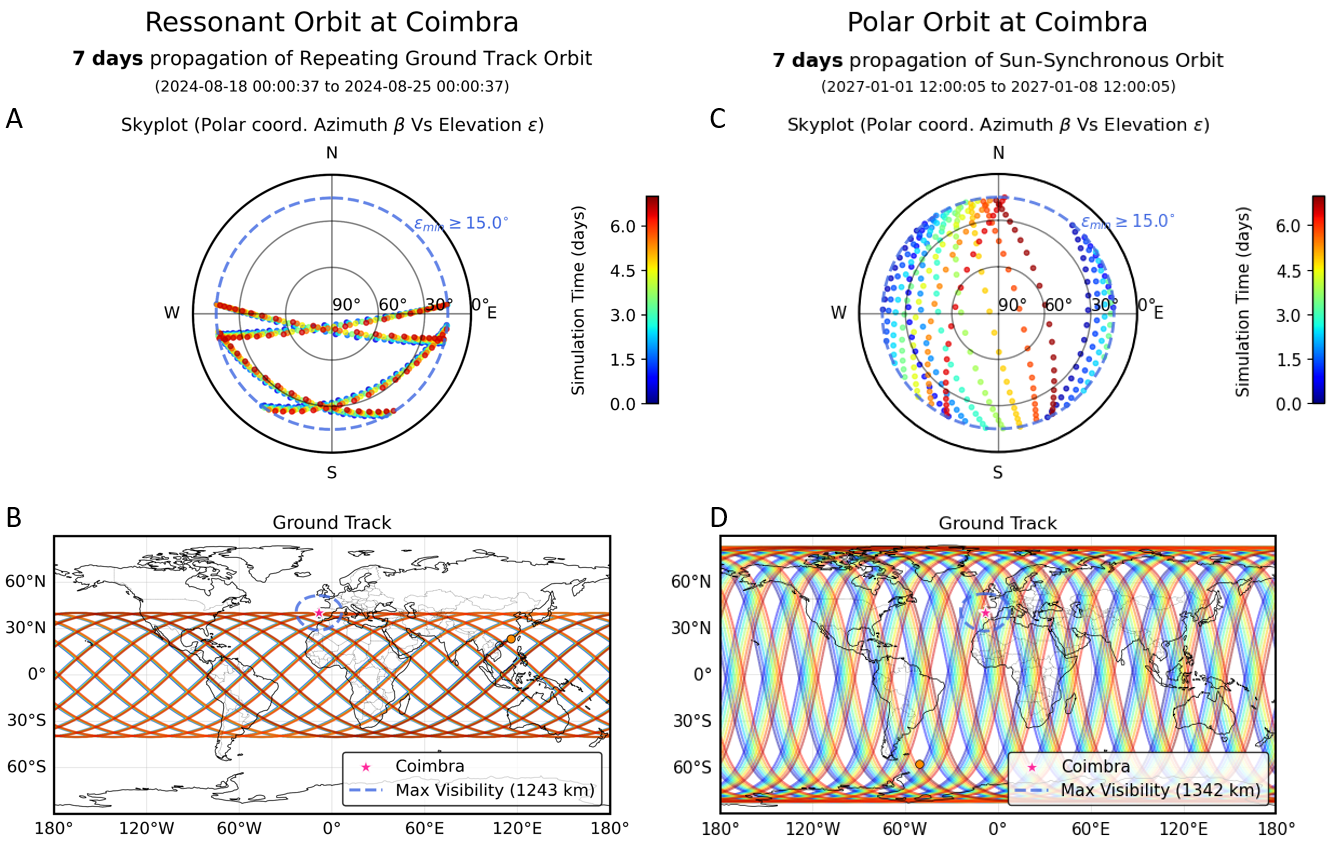
\includegraphics[width=1\linewidth]{images/rgtoVSsso_7days_prop_maps.png}
    \caption{\footnotesize{Plots C and D show the SSO ground track crossing the target latitude at a steep angle (South-North direction) with limited permanence time; on the other hand, plots A and B show the RGTO ground track aligned with the target at Coimbra latitude, maximizing both pass duration and the number of daily revisits. The difference in elevation between the two plots is also evident in the density and geometric distribution of the skyplots. SSO has greater density at low elevations, while RGTO has a more uniform elevation distribution. This has a significant impact on the sensor's effective FOV for achieving observation link access to the ground target.}}
    \label{fig:rgtoVSsso_7day_prop_maps}
\end{figure}


Further details on the necessary sensor trade-off are shown in Figure \ref{fig:rgtoVSsso_7day_prop_old}, which compares the same 7-day propagation RGTO and SSO seeds over Coimbra across three metrics: visibility windows, elevation--distance profile, and off-nadir $\eta$ angle versus Ground Sample Distance (GSD).  The RGTO produces four approximately visible windows with $\eta<60^\circ$ per 24-hour cycle, all exceeding $\varepsilon > 15^{\circ}$ elevation, yielding low off-nadir angles and consequently a GSD well within the mission requirement, totalizing 28 passes over 7 days.  The SSO, governed by its 12-hour repeat cycle, provides only two windows per pass burst at significantly lower elevations, which degrade the observation link geometry and inflate the effective FOV, totalizing 16 passes over 7 days.  
The comparison indicates that approximately 1.75 times as many SSO satellites would be required to match the temporal and spatial coverage delivered by a single RGTO plane. Therefore, the RGTO is preferred for this mission design. 

It is also important to note that SSO orbits are cheaper to reach due to ride-sharing on reusable rockets, and that this orbit is more populated and carries a higher risk of space debris. RGTO can also be achieved with reusable rockets; a trade-off between cost and performance should be made in a future study. For this work, we focus on the best coverage case for the study domain: the RGTO case.

\begin{figure}[H]
    \centering
    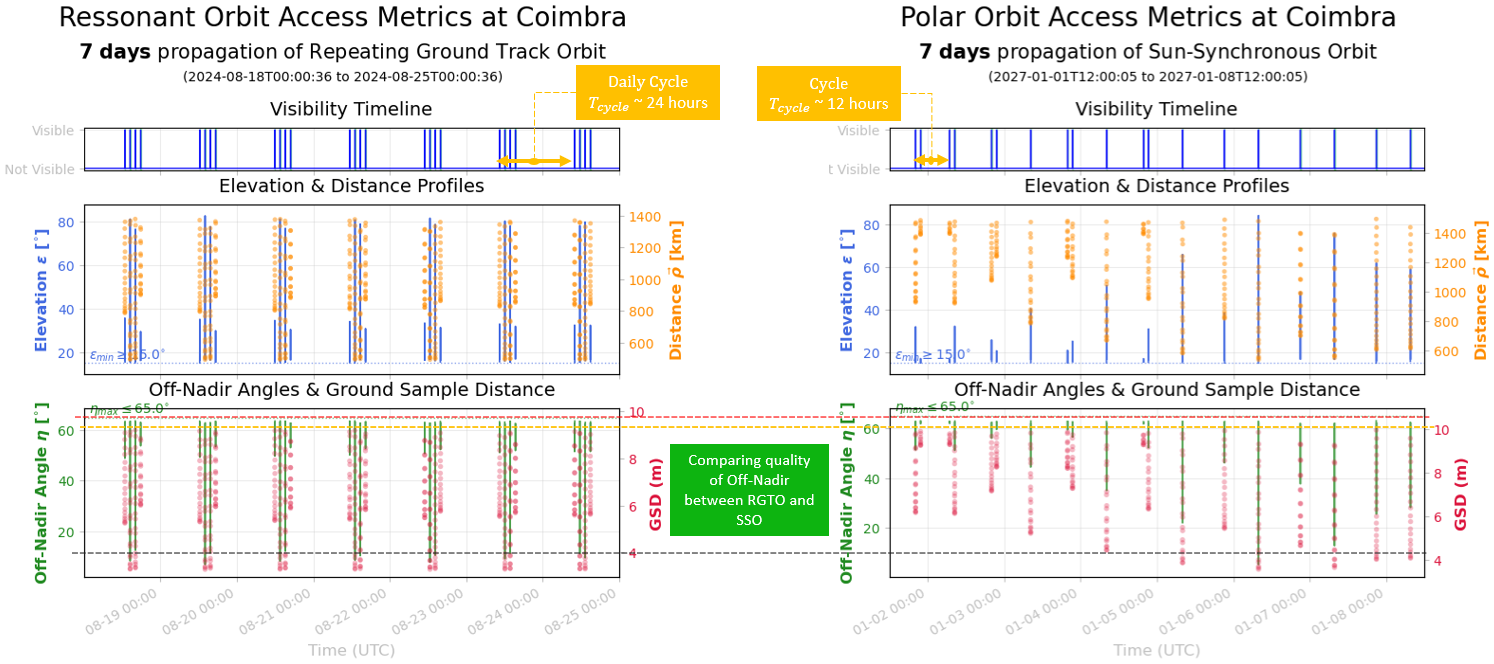
\includegraphics[width=1\linewidth]{images/rgtoVSsso_7days_prop.png}
    \caption{\footnotesize{Observation-link comparison over Coimbra ($\phi_{\text{lat}}=40.2^{\circ}$\,N) for a 7-day propagation.  \textbf{Left column}: RGTO seed ($\tau=15/1$, $h\approx488$\,km, $i=40.2^{\circ}$).  \textbf{Right column}: Sun-Synchronous Orbit (SSO, $h\approx525.8$\,km), $i=97.5^{\circ}$.  \textbf{Row 1}: visibility windows (elevation $\varepsilon$ vs.\ time); \textbf{Row 2}: elevation vs.\ distance; \textbf{Row 3}: off-nadir angle vs.\ GSD.  At $\eta=60^\circ$, the RGTO yields four passes per 24-hour cycle, totalizing 28 passes over 7 days, whereas the SSO with a 12-hour cycle produces for same $\eta$ 16 passes at markedly lower elevation than the RGTO, degrading both coverage continuity and sensor GSD.}}
    \label{fig:rgtoVSsso_7day_prop_old}
\end{figure}
